\documentclass[12pt, oneside]{report}
%\documentclass[12pt, twoside, openany]{report}
%% -------- packages and configuration --------

\usepackage{a4wide}
\usepackage{amsfonts}
\usepackage{amsmath}
\usepackage{enumerate}
\usepackage{verbatim}
\usepackage[T1]{fontenc}
\usepackage[utf8]{inputenc}
\usepackage[MeX]{polski}
\usepackage{amssymb, latexsym}
\usepackage{amsthm}
\usepackage{palatino}
\usepackage{array}
\usepackage{pstricks}
\usepackage{textcomp}
\theoremstyle{definition}
\newtheorem{theorem}{Twierdzenie}[section]
\newtheorem{remark}{Uwaga}[section]
\newtheorem{definition}{Definicja}[section]
\newtheorem{alg}{Algorytm}[chapter]
\newtheorem{prz}{Przypadek}[section]
\newtheorem{np}{Przykład}[section]
\newtheorem{lemma}[theorem]{Lemat}
\newcommand*{\norm}[1]{\left\Vert{#1}\right\Vert}
\newcommand*{\abs}[1]{\left\vert{#1}\right\vert}
\newcommand*{\om}{\omega}
\usepackage{geometry}
\geometry{left=25mm, right=25mm, bindingoffset=10mm, top=25mm, bottom=25mm}
\usepackage{graphicx}
\graphicspath{ {Images/} }
\usepackage[english, polish]{babel}
\usepackage{lmodern}
\usepackage{float}
\usepackage{verbatim}
\usepackage{setspace} 
%\onehalfspacing


\author{Jakub Abelski}
\title{Opracowanie symulatora transportera wahadła odwróconego na wózku}

\begin{document}

%% -------- title page --------
\begin{titlepage}
\pagestyle{empty}
\noindent
\begin{Large}
%\begin{table}[t]
%\centering
%\begin{tabular}[t]{lcr}
% 
\includegraphics[width=70pt,height=70pt]{PW} & POLITECHNIKA WARSZAWSKA & 
\includegraphics[width=70pt,height=70pt]{MiNI}\\
%& WYDZIAŁ MATEMATYKI & \\
%& I NAUK INFORMACYJNYCH &
%\end{tabular}
%\end{table}

\begin{center}
\begin{tabular}{lcr}
	\centering
	\begin{tabular}{c}
		
\includegraphics[width=70pt,height=70pt]{PW}
	\end{tabular} &
	\begin{tabular}{c}
		\small 
		POLITECHNIKA WARSZAWSKA 
		\vspace*{5mm} \\
		\small
		WYDZIAŁ MATEMATYKI \\
		\small
		I NAUK INFORMACYJNYCH 
	\end{tabular} &
	\begin{tabular}{c}
		
\includegraphics[width=70pt,height=70pt]{MiNI}
	\end{tabular}
\end{tabular}
\end{center}

\vfill
\begin{center}PRACA DYPLOMOWA MAGISTERSKA\end{center}
\begin{center}INFORMATYKA\end{center}
\end{Large}

\linespread{1.5}
\begin{center}
\Huge
\textbf{Opracowanie symulatora transportera wahadła odwróconego na wózku}
\end{center}

\begin{center}
\Large
\textbf{Development of simulator for transporter \\of inverted pendulum on a cart}
\end{center}


\vfill
\begin{center}
\Large
Autor:\\
\LARGE Jakub Abelski
\end{center}
\vfill
\begin{center}
\Large
Promotor: prof. dr hab. Krzysztof Marciniak
\end{center}
\vfill
\begin{center}
\large
Warszawa, Grudzień 2016
\end{center}

%% -------- title page reverse --------
\newpage
\hfill
\begin{table}[b]
\centering
\begin{tabular}[t]{ccc}
............................................. & \hspace*{100pt} & .............................................\\
podpis promotora & \hspace*{100pt} & podpis autora
\end{tabular}
\end{table}
\end{titlepage}

%% -------- abstract --------
\setlength{\parindent}{5ex}
\selectlanguage{polish}

\begin{abstract}
Rozwój nowoczesnych technologii opiera się w głównej mierze na usprawnianiu istniejących zasobów oraz poszukiwaniu innowacyjnych rozwiązań. W celu ograniczenia nakładów finansowych, jak również minimalizacji ryzyka popełnienia błędu przy wdrażaniu nowych pomysłów warto rozważyć wykorzystanie narzędzi oferowanych przez środowiska symulacyjne. Komputer potrafi wykryć usterki, z niezwykłą precyzją odpowiedzieć na większość pytań postawionych przez użytkownika, a często daje możliwość wykonania optymalizacji procesu tak, by uzyskać zmaksymalizowany efekt końcowy.

Niniejsza praca wpisuje się w przestawioną retorykę, gdyż poświęcona jest opracowaniu symulatora transportera wahadła odwróconego na wózku. Bazą dla projektu jest dobrze znane zagadnienie dwuwymiarowego układu złożonego z wahadła odwróconego umieszczonego na ruchomej podstawie. Głównym zadaniem systemu jest utrzymanie wahadła w niestabilnym punkcie równowagi i reagowanie na zakłócenia pochodzące z zewnątrz poprzez odpowiedni regulator napięcia na silniku sterującym ruchem podstawy. Prezentowana praca podchodzi do tego zagadnienia w sposób niestandardowy. Wspomniany układ zostaje przeniesiony do świata trójwymiarowego, w którym dwa niezależne systemy związane z kierunkami poziomych osi głównych zostają połączone w jeden moduł sterowania układem. Zabieg ten umożliwia zadanie trajektorii ruchu transportera i przetestowanie skuteczności różnych modeli sterowania położeniem układu i wychyleniem wahadła. Dodatkowym elementem projektu jest uwzględnienie zakłócenia dynamiki w postaci zewnętrznej siły wiatru. Zadaniem transportera jest reagowanie na zakłócenie w taki sposób, by zminimalizować ryzyko stracenia kontroli nad wahadłem. 

Przygotowane rozwiązanie nie posiada jeszcze odzwierciedlenia w technice, natomiast doskonale odnajduje się w świecie symulacji i pozwala na dogłębną analizę pracy układu, jak również wykorzystanie go w grach komputerowych jako wirtualnego pojazdu z nietrywialnym sterowaniem. 

Celem pracy jest zbudowanie uniwersalnego symulatora z konkretną realizacją przedstawionego problemu. Dodatkowym elementem jest możliwość dokonania dogłębnej analizy procesu tworzenia symulacji i wypracowania optymalnego rozwiązania. Ponadto dokument ma na celu ilustrację architektury i ogólnego schematu działania programu, a także przedstawienie wyników przeprowadzonych testów.

Pierwszy rozdział tekstu stanowi bazę teoretyczną dalszych rozważań. Zawiera on podstawowe definicje, przybliża istotę problemu oraz istniejące rozwiązania. Rozdział drugi opisuje logikę systemu. Rozdział trzeci skupia się na opisie rozwiązania: mechanice układu i użytym algorytmom. W czwartym rozdziale omówione zostają testy i porównanie rozwiązań przyjętych w projekcie. Rozdział piąty prezentuje architekturę opracowanego systemu, natomiast rozdział szósty stanowi instrukcję obsługi dla użytkownika. Ostatni rozdział podsumowuje całość pracy, opisuje wnioski oraz przedstawia możliwe kierunki rozwoju systemu.
\end{abstract}

\selectlanguage{english}
\begin{abstract}
Development of new technologies is based mainly on the analysis, improvement of existing resources and finding innovative solutions. Unfortunately, due to financial constraints, as well as the risk of adverse effects it is not recommended to implement the idea without special preparation. In order to significantly reduce the risks using the tools offered by simulation environments should be considered. The computer is able to forgive the mistakes made at the design stage, as well as it can investigate the matter with great precision and answer most of the questions asked by the user. In addition it has the possibility of optimizing processes, so as to obtain the final effect maximized. These arguments leave no doubt that the simulation is an essential element in implementing the new technology.

The thesis is devoted to the development of a simulator for transporter of inverted pendulum on a cart. The project is based on well-known problem of two-dimensional system consisting of an inverted pendulum mounted on a movable platform. The main task of the system is to keep the pendulum in an unstable equilibrium and respond to noises from the environment through the special voltage controller of the platform's engine. The thesis approaches this problem in an innovative way. The system is transferred to a three-dimensional world in which two independent systems associated with the horizontal directions of the principal axes are integrated into a unit. As a result, the movement trajectory can be applied to the system and the pendulum should be transported according to given trajectory. An additional element of the project is adding the wind force. The transporter have to deal with the noise in such a way as to minimize the risk of losing control of the pendulum. 

Prepared solution has not yet reflected in the technique however it perfectly finds itself in the world of simulation. The project allows for in-depth analysis of system's dynamics, as well as it can be used in computer games as a virtual vehicle with non-trivial control.

The aim of the thesis is to build a universal simulator with a concrete realization of the presented problem. An additional element is the possibility of an in-depth analysis of simulation's creation to develop the optimal solution. Furthermore, the document was prepared to illustrate the architecture and general scheme of the system, as well as present the results of tests.

The first chapter is a theoretical basis for further discussion. It includes basic definitions, brings physical background and discusses the existing solutions. The second chapter describes the logic of the whole program. The third chapter focuses on the mechanics of the system and comparison of the solutions adopted in the project. In the fourth and fifth chapter the system architecture and technical documentation are discussed. Chapter six covers manual and tests' description. The last chapter summarizes the whole work. It presents conclusions and future possible directions of development of the system.
\end{abstract}

\selectlanguage{polish}

%% Key words
\newpage
\pagestyle{empty}
\vspace*{\fill}
\begin{center}
\LARGE\textbf{Słowa kluczowe}\\
\end{center}
\begin{center}
Symulacja\\
Transporter\\
Wahadło odwrócone na wózku\\
Dynamika układu\\
Trajektoria ruchu\\
Stabilizacja układu\\
Regulator PID\\
Zakłócenia siłą wiatru \\
Równanie stanu\\
Linearyzacja\\
Algorytm Runge-Kutta
\end{center}
\vspace{\fill}

%% Acknowledgements
\newpage
\pagestyle{empty}
\vspace*{\fill}
\begin{center}
\LARGE\textbf{Podziękowania}\\
\end{center}
Niniejszą pracę pragnę zadedykować rodzicom: Marcie i Janowi Abelskim, dzięki którym miałem możliwość swobodnego kształcenia się i rozwijania swoich zainteresowań.
\vspace{10px}
\\
Chciałbym wyrazić wdzięczność promotorowi: prof. Krzysztofowi Marciniakomwi za jego wsparcie i dobre rady odnośnie kwestii merytorycznych jak i praktycznej części pracy. Specjalne podziękowania dla całej kadry zakładu CAD/CAM na wydziale Matematyki i Nauk Informacyjnych za przekazanie podstaw umożliwiających osiągnięcie odpowiedniego zaawansowania pracy i ugruntowanie wiedzy niezbędnej w przyszłej karierze zawodowej.

\vspace{\fill}

%% -------- table of contents --------
\newpage
\pagestyle{plain}
\setcounter{page}{5}
\tableofcontents

%% -------- chapter I --------
\newpage
\pagestyle{headings}
\hyphenation{Syl-ves-tra}
\hyphenation{Syl-ves-ter-a}

\chapter{Wstęp}
\section{Podstawowe definicje}
\subsection{Symulacja}
Według Słownika Języka Polskiego \cite{PWNSymulacja} symulacja to sztuczne odtwarzanie właściwości danego obiektu lub zjawiska za pomocą jego modelu, natomiast bardzie szczegółowo w zakresie symulacji komputerowej jest to badanie zachowania się obiektów rzeczywistych na podstawie obserwacji działania programów komputerowych symulujących to zachowanie.


Symulację komputerową wykonuje się wtedy, gdy trudno jest wyznaczyć analityczne rozwiązanie problemu lub gdy złożoność systemu uniemożliwia jakąkolwiek ręczną analizę problemu. Symulacja komputerowa wykorzystuje pewien zadany model matematyczny pod postacią kodu programu komputerowego, który jest przetwarzany, a następnie prezentowane są rezultaty.

Symulacja znajduje zastosowania w wielu dziedzinach takich jak:
\begin{itemize}
\item Inżynieria - np. w budownictwie do badania wytrzymałości konstrukcji.
\item Systemy treningowe, gry komputerowe - np. symulatory samolotów, czołgów, statków, itp.
\item Ekonomia i biznes - np. do wyceny instrumentów pochodnych na giełdzie. 
\item Nauki społeczne - np. w badaniu dynamiki populacji.
\item Nauki przyrodnicze - np. w meteorologii do wyznaczania prognozy pogody.
\end{itemize}

\newpage
Kilka przykładów zastosowań symulacji komputerowej przedstawiono na ilustracjach \ref{MeteorologySimulationImage} i \ref{EngineeringSimulationImage}.

\begin{figure}[H]
	\centering
		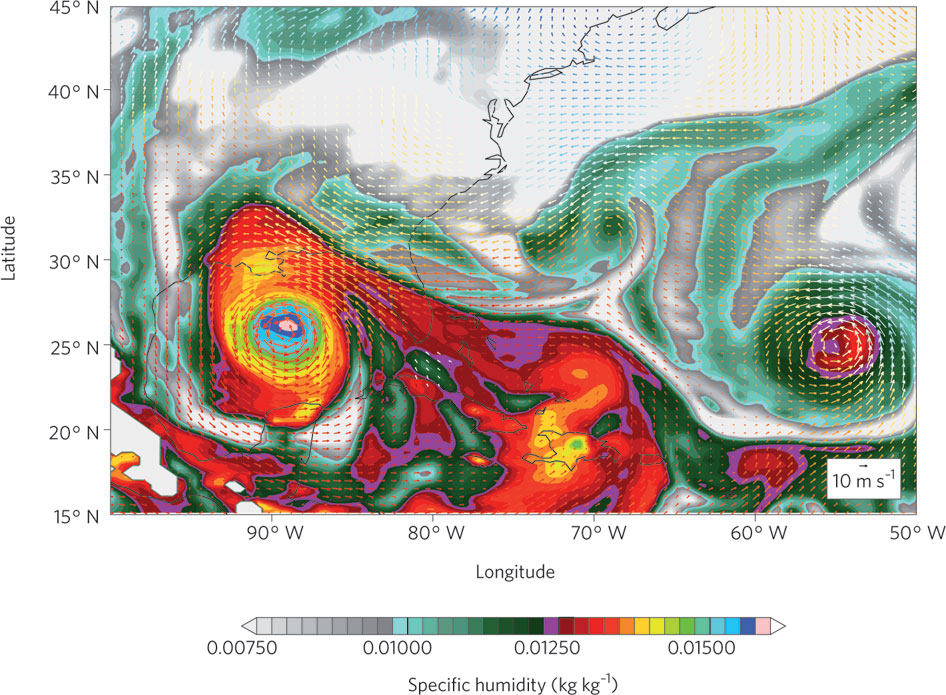
\includegraphics[width = 300pt]{MeteorologySimulation} 
		\caption{\textit{Symulacja dwóch tropikalnych huraganów nad Atlantykiem \cite{MeteorologySimulation}}}
\label{MeteorologySimulationImage}
\end{figure}

\begin{figure}[H]
	\centering
		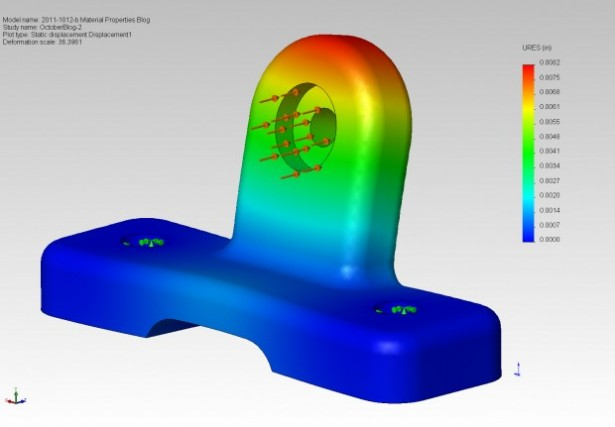
\includegraphics[width = 300pt]{EngineeringSimulation} 
		\caption{\textit{Analiza własności materiału za pomocą symulacji SolidWorks \cite{EngineeringSimulation}}}
\label{EngineeringSimulationImage}
\end{figure}

\newpage
Bazując na \cite{WikiSymulacja} symulacje komputerowe można podzielić ze względu na:
\begin{itemize}
\item Przewidywalność zdarzeń - deterministyczne, gdzie wyniki są powtarzalne i zależne tylko od zadanych parametrów i i interakcji oraz stochastyczne - generowane losowo. 
\item Upływ czasu - ciągły, w którym chwile pośrednie są interpolowane brzegowymi lub dyskretny, gdzie czas zwiększa się przyrostowo.
\item Dane wyjściowe - statyczne, w których wynikiem jest zbiór danych lub dynamiczne, które ukazują cały proces przebiegający w czasie, np. animacja.
\item Zasób komputerów - lokalny lub rozproszony.
\end{itemize}

Przygotowywana praca realizuje symulator z deterministyczną przewidywalnością zdarzeń, czas zwiększa się stałymi przyrostami z możliwością ich modyfikowania. Przetwarzanie systemu odbywa się na pojedynczym komputerze, natomiast dane wyjściowe prezentowane są w postaci dynamicznej animacji.

\subsection{Układ dynamiczny}
\subsubsection{Wprowadzenie}
Układ dynamiczny jest to matematyczny model zjawiska występującego w przyrodzie, określany poprzez funkcję zachowania układu w danym czasie. Model ten jest zwykle opisany poprzez układ równań różniczkowych, zwanych równaniem stanu. W danej jednostce czasowej system posiada stan wyrażony jako wektor liczb utożsamiany z punktem w przestrzeni stanu. Ewolucja układu polega na wyznaczaniu kolejnych stanów na podstawie poprzednich poprzez użycie funkcji przejścia. Funkcja ta może być deterministyczna lub stochastyczna. W pierwszym przypadku dla zadanego czasu stan wyznaczany jest jednoznacznie, w drugim przypadku na ewolucję układu wpływają dodatkowe zdarzenia losowe (przytoczone zagadnienie zostało szerzej omówione w \cite{MarciniakDynamicSystems}).

\subsubsection{Wahadło odwrócone na wózku}
Niniejsza praca skupia się na modelu dynamiki układu złożonego z wahadła odwróconego umieszczonego na ruchomej platformie. Wahadło odwrócone jest rodzajem wahadła, w którym środek masy znajduje się powyżej punktu zaczepienia. Wahadło połączone jest z wózkiem, który porusza się w płaszczyźnie poziomej za pomocą silnia napędowego. Przykładowy układ pokazany został na ilustracji \ref{SystemModelImage}.

\begin{figure}[H]
	\centering
		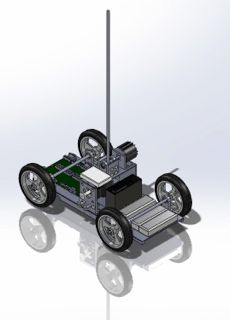
\includegraphics[width = 100pt]{SystemModel} 
		\caption{\textit{Model bezprzewodowego układu mechanicznego dla odwróconego wahadła na wózku \cite{SystemModel}}}
		\label{SystemModelImage}
\end{figure}

Przedstawione ustawienie wahadła powoduje, że znajduje się ono w niestabilnym punkcie równowagi. Punkt równowagi jest miejscem przy którym element pozostaje w bezruchu (prędkość zmiany stanu jest zerowa). Wyróżniamy stabilnie i niestabilne punkty równowagi. Wahadło posiada dwa punkty równowagi: stabilne znajdujące się poniżej punktu zaczepienia i niestabilnie powyżej punktu równowagi. W przypadku drugiego z nich nawet niewielkie zaburzenie stanu układu wywołuje ruch wahadłowy, który ustaje dopiero po zatrzymaniu się w stabilnym punkcie równowagi. 


Układ będący przedmiotem zainteresowania pokazany został na schemacie \ref{SytemSchemeImage}.

\begin{figure}[H]
	\centering
		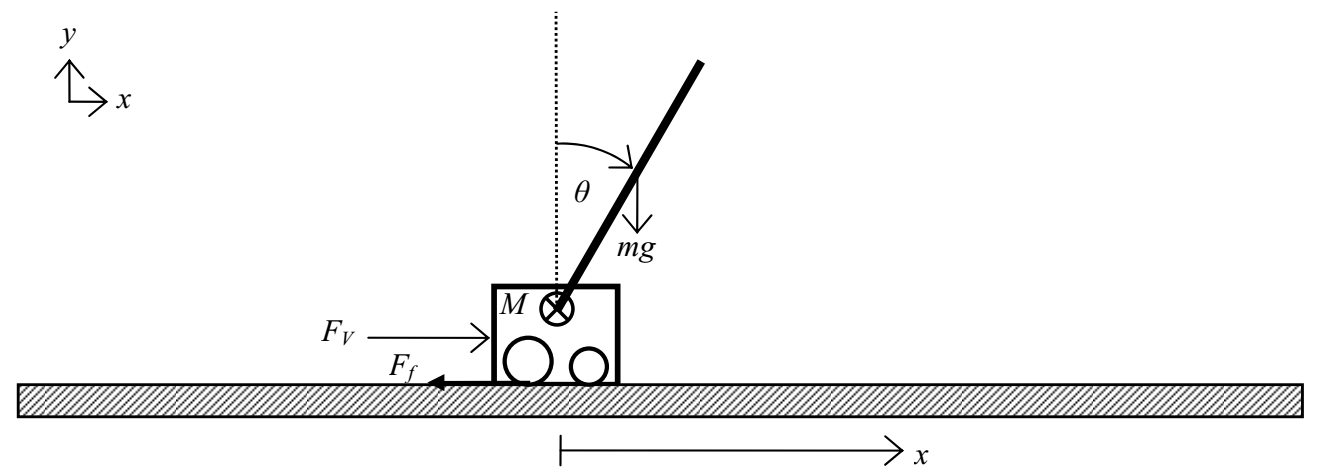
\includegraphics[width = 300pt]{SystemScheme} 
		\caption{\textit{Uproszczony schemat fizyki układu wahadła odwróconego na wózku \cite{LIMP} }}
		\label{SytemSchemeImage}
\end{figure}

Najważniejsze elementy schematu:
\begin{itemize}
\item \(F_v\) - siła napędowa wózka \([N]\).
\item \(F_f\) - siła tarcia \([N]\).
\item \(m\) - masa wahadła \([kg]\). 
\item \(M\) - masa wózka \([kg]\).
\item \(g\) - przyspieszenie ziemskie \([\frac{m}{s^2}]\) 
\item \(\theta\) - kąt między osią wahadła a pionową osią układu \([rad]\).
\end{itemize}

Stan układu określany jest poprzez cztery parametry:
\begin{itemize}
\item Położenie środka wózka w osi X.
\item Prędkość liniowa wózka.
\item Kąt odchylenia wahadła od osi pionowej.
\item Prędkość kątowa wahadła.
\end{itemize}

Parametry fizyczne układu (wraz z nominalnymi wartościami opracowanymi na podstawie literatury \cite{LIMP}) pokazane zostały w poniższej tabeli:
\begin{center}
\begin{tabular}{|c|c|}
  \hline 
  Parametr & Wartość\\
  \hline
  masa wózka & 0.79 \(kg\) \\
  \hline
  masa wahadła & 0.23 \(kg\) \\
  \hline
  długość wahadła & 0.61 \(m\) \\
  \hline
  współczynnik tarcia wózka & 7.68 \(\frac{N}{ms^{-1}}\) \\
  \hline
  współczynnik konwersji napięcia na siłę & 1.72 \(\frac{N}{V}\) \\
  \hline
\end{tabular} 
\end{center}

Podstawowym zagadnieniem związanym z omawianym układem jest kontrola wychylenia wahadła. Urządzenie sterujące poprzez przyłożenie odpowiedniego napięcia na silniku wywołuje siłę napędową, która porusza platformą. Odpowiedni ruch podstawy pozwala na utrzymanie wahadła w punkcie równowagi.

\subsubsection{Trójwymiarowa wersja układu}
Dwuwymiarowy układ wahadła odwróconego na wózku można wykorzystać do zbudowania trójwymiarowego odpowiednika. Nowy model składa się z dwóch podukładów odpowiedzialnych za płaszczyzny związane z osiami głównymi układu, odpowiednio: O(XZ) i O(YZ). Przybliżony model znajduje się na rysunku \ref{3DimModel}

\begin{figure}[H]
	\centering
		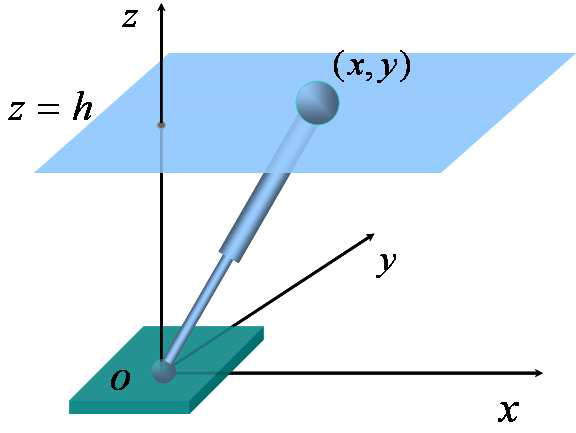
\includegraphics[width = 200pt]{3DimModel} 
		\caption{\textit{Uproszczony schemat trójwymiarowego układu wahadła odwróconego na wózku \cite{3DimModel}}}
		\label{3DimModel}
\end{figure}

Wynikowy stan całego układu jest sumą stanów poszczególnych komponentów. Ruch trójwymiarowego modelu wyznaczany jest jako złożenie (superpozycja) ruchów podukładów. Kierunek wychylenia wahadła można wyznaczyć za pomocą elementarnych własności geometrycznych. 

Opracowany w ten sposób model pozwala na poruszanie układem po płaszczyźnie O(XY). Wykorzystując odpowiednie narzędzie sterujące można dokonać stabilizacji układu nie tylko dla kąta odchylenia wahadła, ale również pozycji wózka na płaszczyźnie.

\section{Opis problemu}
\subsection{Motywacja}
Opracowywane zagadnienie jest nietrywialną modyfikacją dobrze znanego zagadnienia sterowania wahadłem odwróconym na wózku. Wybrana tematyka pracy magisterskiej jest ściśle związana z zainteresowaniami autora oraz materiałem realizowanym w ramach studiów. Przygotowanie pracy daje możliwość pogłębienia wiedzy z zakresu układów dynamiki i teorii sterowania. Dodatkowo pozwala na zmierzenie się z problemem wykonania symulacji, która w profesjonalny sposób zrealizuje zadane zagadnienie, a dodatkowo będzie atrakcyjna dla użytkownika końcowego. Ponadto wypracowana koncepcja systemu nie posiada jeszcze odzwierciedlenia we współczesnej technice. Toteż ze względu na elementy innowacyjności rozwiązania, pomysł ten jest okazją do analizy niestandardowego systemu, który może mieć zastosowanie w przyszłości, przynajmniej w środowisku wirtualnym.

\subsection{Główne cele}
Podstawowym celem pracy jest opracowanie symulatora transportera wahadła odwróconego na wózku. Zagadnienie to można w naturalny sposób podzielić na kilka podproblemów, co pozwala na szczegółowy przegląd poszczególnych elementów:
\begin{itemize}
\item Układ wahadła odwróconego na wózku. Projekt opiera się na analizie prostego modelu fizycznego wraz z implementacją jego zachowania. Dodatkowo rozszerza podstawową, dwuwymiarową wersję, na układ trójwymiarowy, by zwiększyć poziom skomplikowania, ocenić użyteczność zaproponowanego pomysłu i wzbogacić efekt końcowy. Dodatkowym elementem jest wprowadzenie zakłóceń do układu w postaci podmuchów powietrza. Istotny jest również przegląd przypadków szczególnych i wypracowanie odpowiedniej reakcji na ich zaistnienie. Projekt powinien w pełni przedstawić zadane zagadnienie, wraz z możliwością wprowadzania modyfikacji układu i pełnym podglądem na jego stan. Dysponując w pełni zaimplementowanym modelem bazowym można badać zachowanie układu wobec zadanych parametrów wejściowych i dynamicznych.
\item Stabilizacja układu. Naturalnym zagadnieniem wiążącym się z układem wahadła odwróconego na wózku jest próba stabilizacji wychylenia wahadła w obrębie pionowej osi układu tak, by komponent pozostawał w niestabilnym punkcie równowagi. Celem projektu jest zrealizowanie wspomnianej stabilizacji za pomocą regulacji napięcia podawanego na wejście do silników sterujących wózkiem. Zadanie to wymaga wykorzystania wiedzy z zakresu teorii sterowania, w szczególności pojęcia regulatora. Praca powinna oprzeć się na implementacji odpowiedniego regulatora i przetestowaniu jego działania względem poszczególnych parametrów systemu. 
\item Transport układu. Osiągnięcie kontroli nad wychyleniem wahadła pozwala na dalsze rozszerzanie funkcjonalności systemu. Kolejnym etapem projektu jest stworzenie modułu sterującego ruchem całego układu. System powinien umożliwić stworzenie dowolnej trajektorii ruchu lub wczytanie przygotowanego przykładu, a następnie zmuszenie układu fizycznego do odwzorowania zadanej ścieżki ruchu.
\item Opracowanie symulatora. System nie będzie użyteczny, jeśli nie zostanie zaprezentowany użytkownikowi końcowemu w wygodnej i atrakcyjnej wizualnie formie. Ostatnim istotnym celem projektu jest stworzenie aplikacji na komputer, której zadaniem będzie wizualizacja zachowania całego układu fizyki. Ponadto program powinien posiadać intuicyjny panel sterowania oraz dostarczać na bieżąco pełnej informacji na temat stanu sytemu. Dodatkowym walorem aplikacji może być tryb interakcyjny, który pozwoli użytkownikowi nie tylko na przegląd mechaniki układu, lecz również na zabawę w sterowanie pojazdem.
\end{itemize}

\section{Przegląd istniejących rozwiązań}
\subsection{Symulatory}
W obecnych czasach oprogramowanie symulacyjne jest podstawą funkcjonowania wielu gałęzi przemysłu. Przed przystąpieniem do realizacji projektu autor skupił się na przeglądzie najbardziej popularnych narzędzi symulacyjnych w celu znalezienia kluczowych cech, jakie powinien spełniać dobry symulator. Na szczególną uwagę zasługują trzy rozwiązania:
\begin{itemize}
\item Simulink - pakiet numeryczny MATLAB firmy The MathWorks służący do przeprowadzania symulacji komputerowych. Narzędzie pozwala na tworzenie modeli poprzez wybór komponentów z interfejsu graficznego. Zapewnia symulację z czasem dyskretnym i ciągłym. Simulink wykorzystywany jest głównie do cyfrowego przetwarzania sygnałów, teorii sterowania i analizy obwodów elektrycznych.
\item LabVIEW - środowisko programistyczne firmy National Instruments skupiające się głównie na pomiarach i analizie danych. Pozwala na tworzenie modeli poprzez specjalny graficzny język programowania. LabVIEW znajduje zastosowanie w ośrodkach badawczych i testach przemysłowych.
\item SolidWorks Simulation - pakiet symulacyjny będący częścią programu komputerowego typu CAD firmy Dassault Systèmes. Umożliwia analizę modeli pod wieloma kątami technicznym, symulację ruchu układu w obecności różnych czynników zewnętrznych. Narzędzie wykorzystywane przez wiodące firmy zajmujące się przemysłem.  
\end{itemize}

Przytoczone przykłady zostały zanalizowane pod kątem budowy, możliwości technicznych, sposobu prezentacji danych i interakcji z użytkownikiem. Wypracowane wnioski dały gruntowną podstawę do stworzenia własnego rozwiązania opartego na kilku najważniejszych cechach dobrej symulacji:
\begin{itemize}
\item Modularna budowa - program powinien być zbudowany z respektowaniem standardów inżynierii oprogramowania. Poszczególne funkcjonalności powinny być wyodrębnione i tworzyć pojedyncze pakiety, które będzie można wykorzystywać jako samodzielne elementy.
\item Prostota - konkretne narzędzie powinno spełniać wszystkie wymagania techniczne i ukazywać rezultaty w jak najbardziej przejrzysty sposób. Dodatkowe elementy powodują jedynie przesłonięcie kluczowych funkcjonalności.
\item Dostęp do danych - symulacja powinna w każdej chwili udostępniać komplet niezbędnych danych fizycznych, wizualizować stan zadanego układu oraz gromadzić istotne parametry w formie wykresów lub diagramów.
\item Sterowanie - modyfikacja parametrów symulacji powinna być intuicyjna dla każdego użytkownika.
\end{itemize}
\subsection{Dynamika i sterowanie}
Zagadnienie stabilizacji dwuwymiarowego układu wahadła odwróconego na wózku zostało szeroko omówione w wielu pracach naukowych. Ze względu na prostotę podstawowego modelu temat ten często pojawia się jako materiał na laboratorium na studiach poświęconych automatyce i robotyce (przykładem jest instrukcja \cite{LIMP}).

Dokładna analiza problemu opiera się na wyborze jednego z dwóch modeli: nieliniowego lub zlinearyzowanego. W pierwszym przypadku model wiernie odwzorowuje zachowanie wahadła niezależnie od jego wychylenia, w drugim pojawia się ograniczenie na nieznaczne wychylenia wahadła. Większość przeanalizowanych prac realizuje drugie założenie ze względu na znaczne uproszczenia obliczeń. Kolejnym wyróżnikiem jest sposób stabilizacji układu. Istnieje wiele narzędzi z zakresu teorii sterowania, które pozwalają na kontrolowanie układu. Najbardziej popularnymi są regulatory: PID i LQR. Szczegółowy przegląd i porównanie narzędzi zostało omówione w artykule \cite{OptimalControl}. Autor pracy skupił się wyłącznie na sterowaniu regulatorem PID, jednakże pozostawił możliwość zamiany kontrolera na dowolny inny.

Zagadnienie trójwymiarowe znajduje swoje odniesienie jedynie w modelowaniu poruszania dwunożnego robota, w którym skomplikowany model zostaje zastąpiony wahadłem. Stabilizacja uproszczonego modelu pozwala na poruszanie robotem przy zachowaniu stabilności jego postawy. Temat został gruntownie przedstawiony w artykule \cite{BipedWalking}.

Symulacja transportera układu nie jest zagadnieniem szeroko omówionym, toteż autor oparł rozwiązanie na ogólnej wiedzy z zakresu dynamiki układów i sterowania. 


%% -------- chapter II --------
\newpage
\chapter{Definicja projektu}
\section{Zakres projektu}
Projekt obejmuje opracowanie biblioteki fizyki dla transportera wahadła odwróconego na wózku oraz symulatora wizualizującego działanie biblioteki. Aplikacja przeznaczona jest na platformę Windows.

Projekt podzielony jest na kilka głównych elementów:
\begin{itemize}
\item Budowa dynamiki układu w oparciu o podstawy matematyczno-fizyczne.
\item Opracowanie modułu kontroli układem w celu zapewnienia stabilności.
\item Wprowadzenie modułu zakłóceń w postaci siły wiatru.
\item Obsługa trajektorii ruchu.
\item Wizualizacja układu na trójwymiarowej scenie.
\item Zarządzanie animacją i modyfikacja parametrów układu.
\item Umożliwienie użytkownikowi ręcznej kontroli systemu poprzez tryb gry.
\end{itemize}

\section{Analiza wymagań}
Wymagania względem projektu można podzielić na funkcjonalne i niefunkcjonalne. Pierwsze odnoszą się do konkretnych zadań, jakie aplikacja powinna realizować. Drugie dotyczą ogólnych cech jakimi program powinien się charakteryzować.

Podstawowe wymagania niefunkcjonalne:
\begin{itemize}
\item Użyteczność - program powinien w pełni realizować postawione zadania, a dodatkowo zachęcać użytkownika do zrozumienia tematyki.
\item Stabilność - aplikacja powinna działać poprawnie bez względu na interakcję użytkownika.
\item Łatwość użytkowania - korzystanie z funkcjonalności powinno być intuicyjne, ponadto wszystkie najważniejsze informacje powinny zostać zebrane w charakterze pomocy.
\item Łatwość modyfikowania - program powinien umożliwiać dostosowywanie ustawień w zależności od potrzeb użytkownika. 
\item Modularność - każdy element systemu powinien być skonstruowany jako oddzielny moduł udostępniający szereg funkcji.
\item Rozszerzalność - kod źródłowy aplikacji powinien być przejrzysty, łatwy do zarządzania i rozszerzalny.
\end{itemize}

Najważniejsze wymagania funkcjonalne:
\begin{itemize}
\item Zarządzanie aplikacją
\begin{itemize}
\item Wybór jednego z trybów działania aplikacji (podstawowy, śledzenie trajektorii, tryb gry).
\item Modyfikacja parametrów startowych układu.
\item Możliwość ustawienia aktualnego regulatora i generatora wiatru.
\item Modyfikacja dokładności śledzenia trajektorii.
\item Zarządzanie parametrami wiatru w trakcie przebiegu animacji.
\item Wybór trajektorii z zestawu przygotowanych przykładów.
\item Możliwość stworzenia nowej trajektorii poprzez zadanie jej parametryzacji.
\end{itemize}
\item Wizualizacja
\begin{itemize}
\item Trójwymiarowa scena z możliwością swobodnej manipulacji kamerą.
\item Umieszczenie modelu transportera w postaci platformy na kołach z przyczepionym odwróconym wahadłem.
\item Wyświetlanie płaszczyzny, po której porusza się model, wraz z podziałką metryczną. 
\item W zależności od ustawień wyświetlania pokazywanie trajektorii ruchu wahadła i wózka.
\item Kontrolowanie postępu animacji poprzez odpowiedni panel.
\item Możliwość przełączania wyświetlania między trybami: prostych kolorów i tekstur.
\item Możliwość ręcznego sterowania układem za pomocą myszy i klawiatury.
\end{itemize}
\item Prezentacja danych
\begin{itemize}
\item Dynamiczne wykresy dla kluczowych danych, tj. błąd regulacji czy podawane napięcie na silniku.
\item Możliwość zapisywania aktualnie wygenerowanych wykresów.
\item Wyświetlanie aktualnego stanu układu.
\item Prezentacja informacji ogólnych na temat aplikacji i dynamiki układu oraz interaktywnej pomocy.
\end{itemize}
\end{itemize}

\section{Ograniczenia}
W trakcie wstępnej analizy projektu przyjęto zestaw ograniczeń w celu zachowania spójności pracy i uniknięcia nadmiernego rozszerzania mniej istotnych elementów. Są to:
\begin{itemize}
\item Konieczność spełnienia wszystkich podstawowych wymagań wymienionych w poprzedniej sekcji.
\item Możliwość uproszczenia modelu w celu zmniejszenia złożoności obliczeń.
\item Ograniczenie realizacji stabilizacji układu do użycia różnych odmian regulatora PID.
\item Ograniczenie jakości wizualizacji do wyświetlania prostego modelu układu na trójwymiarowej scenie.
\end{itemize}

%% -------- chapter III --------
\newpage
\chapter{Opis rozwiązania}
\section{Podstawy matematyczno-fizyczne}
\subsection{Równanie stanu}
\subsection{Algorytm Rungego-Kutty}
\subsection{Regulator PID}
\subsection{Regulator podwójny PID}
\section{Mechanika systemu}
\subsection{Model matematyczny ruchu}
\subsection{Linearyzacja modelu}
\subsection{Stabilizacja układu}
\subsection{Wprowadzenie zakłóceń do modelu}
\subsection{Wprowadzenie trajektorii ruchu}
\subsection{Regulacja ruchu względem zadanej trajektorii}
\section{Rozwiązywanie równań mechaniki systemu}
\subsection{Algorytmy}


%% -------- chapter IV --------
\chapter{Testy i porównanie przyjętych rozwiązań}
\section{Stabilizacja układu}
\section{Ruch po trajektorii}
\section{Wpływ parametrów układu na jego zachowanie}
\section{Testowanie przypadków szczególnych}


%% -------- chapter V --------
\chapter{Architektura systemu}
\section{Ogólny opis rozwiązania}
\section{Wykorzystane narzędzia}
\subsection{Windows Presentation Foundation}
\subsection{HelixToolkit}
\subsection{OxyPlot}
\subsection{Pozostałe}
\section{Wzorce projektowe}
\section{Komponenty aplikacji}
\subsection{Modele}
\subsection{Kontrolery}
\section{Zarządzanie aplikacją}


%% -------- chapter VI --------
\chapter{Instrukcja użytkownika}
\section{Panel kontrolny}
\subsection{Moduły}
\subsection{Opcje}
\subsection{Sterowanie parametrami}
\section{Wizualizacja}
\subsection{Scena}
\subsection{Wykresy}
\subsection{Podgląd stanu}
	
%% -------- chapter VII --------
\newpage
\chapter{Podsumowanie pracy}
\section{Ocena rozwiązania}
\subsection{Stopień realizacji projektu}
\subsection{Poprawność rozwiązania}
\section{Krytyczna refleksja}
\section{Możliwości rozszerzania projektu}

	
%% -------- bibliography --------
\pagestyle{plain}
\begin{thebibliography}{11}

\bibitem{MarciniakDynamicSystems} Marciniak K., \emph{Dynamic systems}, w: \emph{Modelling in state space}, Warszawa, 2003.

\bibitem{MarciniakClosedLoop} Marciniak K., \emph{Design of Closed loop control}, w: \emph{Modelling in state space}, Warszawa, 2003.

\bibitem{MarciniakControlSystems} Marciniak K., \emph{Control systems}, w: \emph{Modelling in state space}, Warszawa, 2003.

\bibitem{LIMP} Robles R., Shardt Y., \emph{Linear motion inverted pendulum, derivation of the state-space model}
\\*
http://www.jtjt.pl/www/pages/odwrocone-wahadlo/LMIP.pdf

\bibitem{JTJT} Tyma J., \emph{Odwrócone wahadło}
\\*
http://www.jtjt.pl/odwrocone-wahadlo

\bibitem{PWNSymulacja} \emph{Słownik Języka Polskiego}
\\*
http://sjp.pwn.pl

\bibitem{WikiSymulacja} \emph{Symulacja komputerowa},
\\*
https://pl.wikipedia.org/wiki/Symulacja\_komputerowa

\bibitem{MeteorologySimulation} Hawkins E., Vidale P. \emph{Two tropical Atlantic hurricanes in a high-resolution atmospheric simulation with the HadGEM3 global climate model at a resolution of N512}, 27.07.2012,
\\*
http://www.nature.com/nclimate/journal/v2/n8/fig\_tab/nclimate1639\_F1.html

\bibitem{EngineeringSimulation} 3DVision Technologies \emph{The Importance of Material Properties in Analysis with SolidWorks Simulation}, 18.05.2012
\\*
http://blogs.solidworks.com/solidworksblog/2012/05/material-properties-in-\\analysis.html

\bibitem{SystemModel} \emph{Wireless Inverted Pendulum Cart},
\\*
http://www.mne.k-state.edu/static/nlc/tiki-index.php?page=\\S\_H\_WirelessInvertedPendulumCart

\bibitem{3DimModel}  \emph{Project: Gait Pattern Generation},
\\*
http://www.wrighteagle.org/en/research/projgait.php

\bibitem{BipedWalking} Kajita S., \emph{The 3D Linear Inverted Pendulum Mode: A simple modeling for a biped walking pattern generation}, 2001

\bibitem{OptimalControl} Prasad L., \emph{Optimal Control of Non linear Inverted Pendulum Dynamical System with Disturbance Input using PID Controller \& LQR}, 2011

\end{thebibliography}


%% -------- statement --------
\selectlanguage{polish}
\clearpage
\pagestyle{empty}
\noindent Warszawa, dnia \today
\vspace{5cm}
\begin{center}
	\LARGE{Oświadczenie}
\end{center}
Oświadczam, że pracę magisterską pod tytułem: ,,Opracowanie symulatora transportera wahadła odwróconego na wózku'', której promotorem jest prof. dr hab. Krzysztof Marciniak, wykonałem samodzielnie, co poświadczam własnoręcznym podpisem.
\vspace{2cm}
\begin{flushright}
...........................................
\end{flushright}

\end{document}

